\documentclass{standalone}

\usepackage{tikz}
\usetikzlibrary{decorations.pathreplacing,positioning, arrows.meta}

\begin{document}         
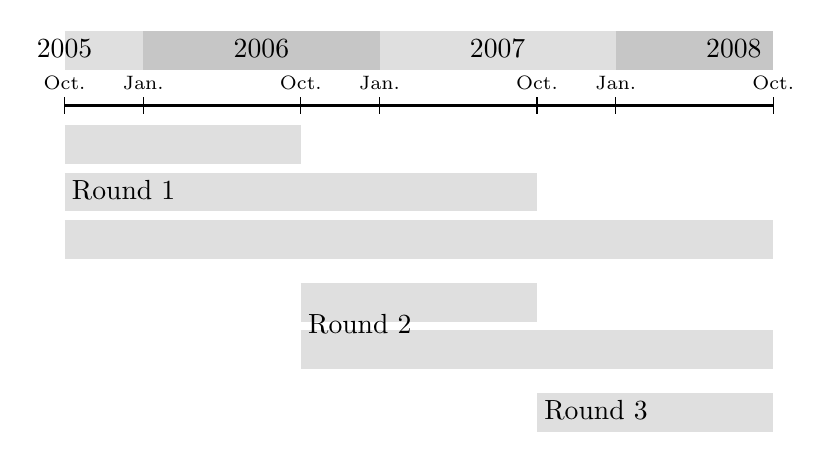
\begin{tikzpicture}

% draw horizontal line   
\draw[thick] (-1,0) -- (8,0) node[font=\normalsize,below left=3pt and -8pt]{};

% draw vertical lines
\foreach \x in {-1,0,2,3,5,6,8}
\draw (\x cm,3pt) -- (\x cm,-3pt);

% CALENDAR
\foreach \x/\perccol in
{-1/50,0/90,1/90,2/90,3/50,4/50,5/50,6/90,7/90}
\draw[lightgray!\perccol!white, line width=14pt] 
(\x,.7) -- +(1,0);

% dates
\foreach \x/\descr in {-1/2005,{1.5}/2006,{4.5}/2007,{7.5}/2008}
\node[font=\normalsize, text height=1.75ex, text depth=.5ex] at (\x,.7) {{\descr}};
\foreach \x/\descr in {-1/{Oct.},0/{Jan.},2/{Oct.},3/{Jan.},5/{Oct.},6/{Jan.},8/{Oct.}}
\node[font=\scriptsize, text height=1.75ex, text depth=.5ex] at (\x,.3) {{\descr}};


% ROUND 1
% Age 1
\foreach \x/\perccol in
{-1/50,0/50,1/50}
\draw[lightgray!\perccol!white, line width=14pt] 
(\x,-.5) -- +(1,0);

% Age 2
\foreach \x/\perccol in
{-1/50,0/50,1/50,2/50,3/50,4/50}
\draw[lightgray!\perccol!white, line width=14pt] 
(\x,-1.1) -- +(1,0);

% Age 3
\foreach \x/\perccol in
{-1/50,0/50,1/50,2/50,3/50,4/50,5/50,6/50,7/50}
\draw[lightgray!\perccol!white, line width=14pt] 
(\x,-1.7) -- +(1,0);

% ROUND 2
% Age 1
\foreach \x/\perccol in
{2/50,3/50,4/50}
\draw[lightgray!\perccol!white, line width=14pt] 
(\x,-2.5) -- +(1,0);

% Age 2
\foreach \x/\perccol in
{2/50,3/50,4/50,5/50,6/50,7/50}
\draw[lightgray!\perccol!white, line width=14pt] 
(\x,-3.1) -- +(1,0);

% ROUND 3
% Age 1
\foreach \x/\perccol in
{5/50,6/50,7/50}
\draw[lightgray!\perccol!white, line width=14pt] 
(\x,-3.9) -- +(1,0);


\node [font=\normalsize, text height=1.75ex, text depth=.5ex] at (-.25,-1.1) {Round 1};
\node [font=\normalsize, text height=1.75ex, text depth=.5ex] at (2.75,-2.8) {Round 2};
\node [font=\normalsize, text height=1.75ex, text depth=.5ex] at (5.75,-3.9) {Round 3};
\end{tikzpicture}

\end{document}
